
\chapter{Related Work}
\label{chapter:Related_Work}

\begin{figure}[h!]
  \centering
    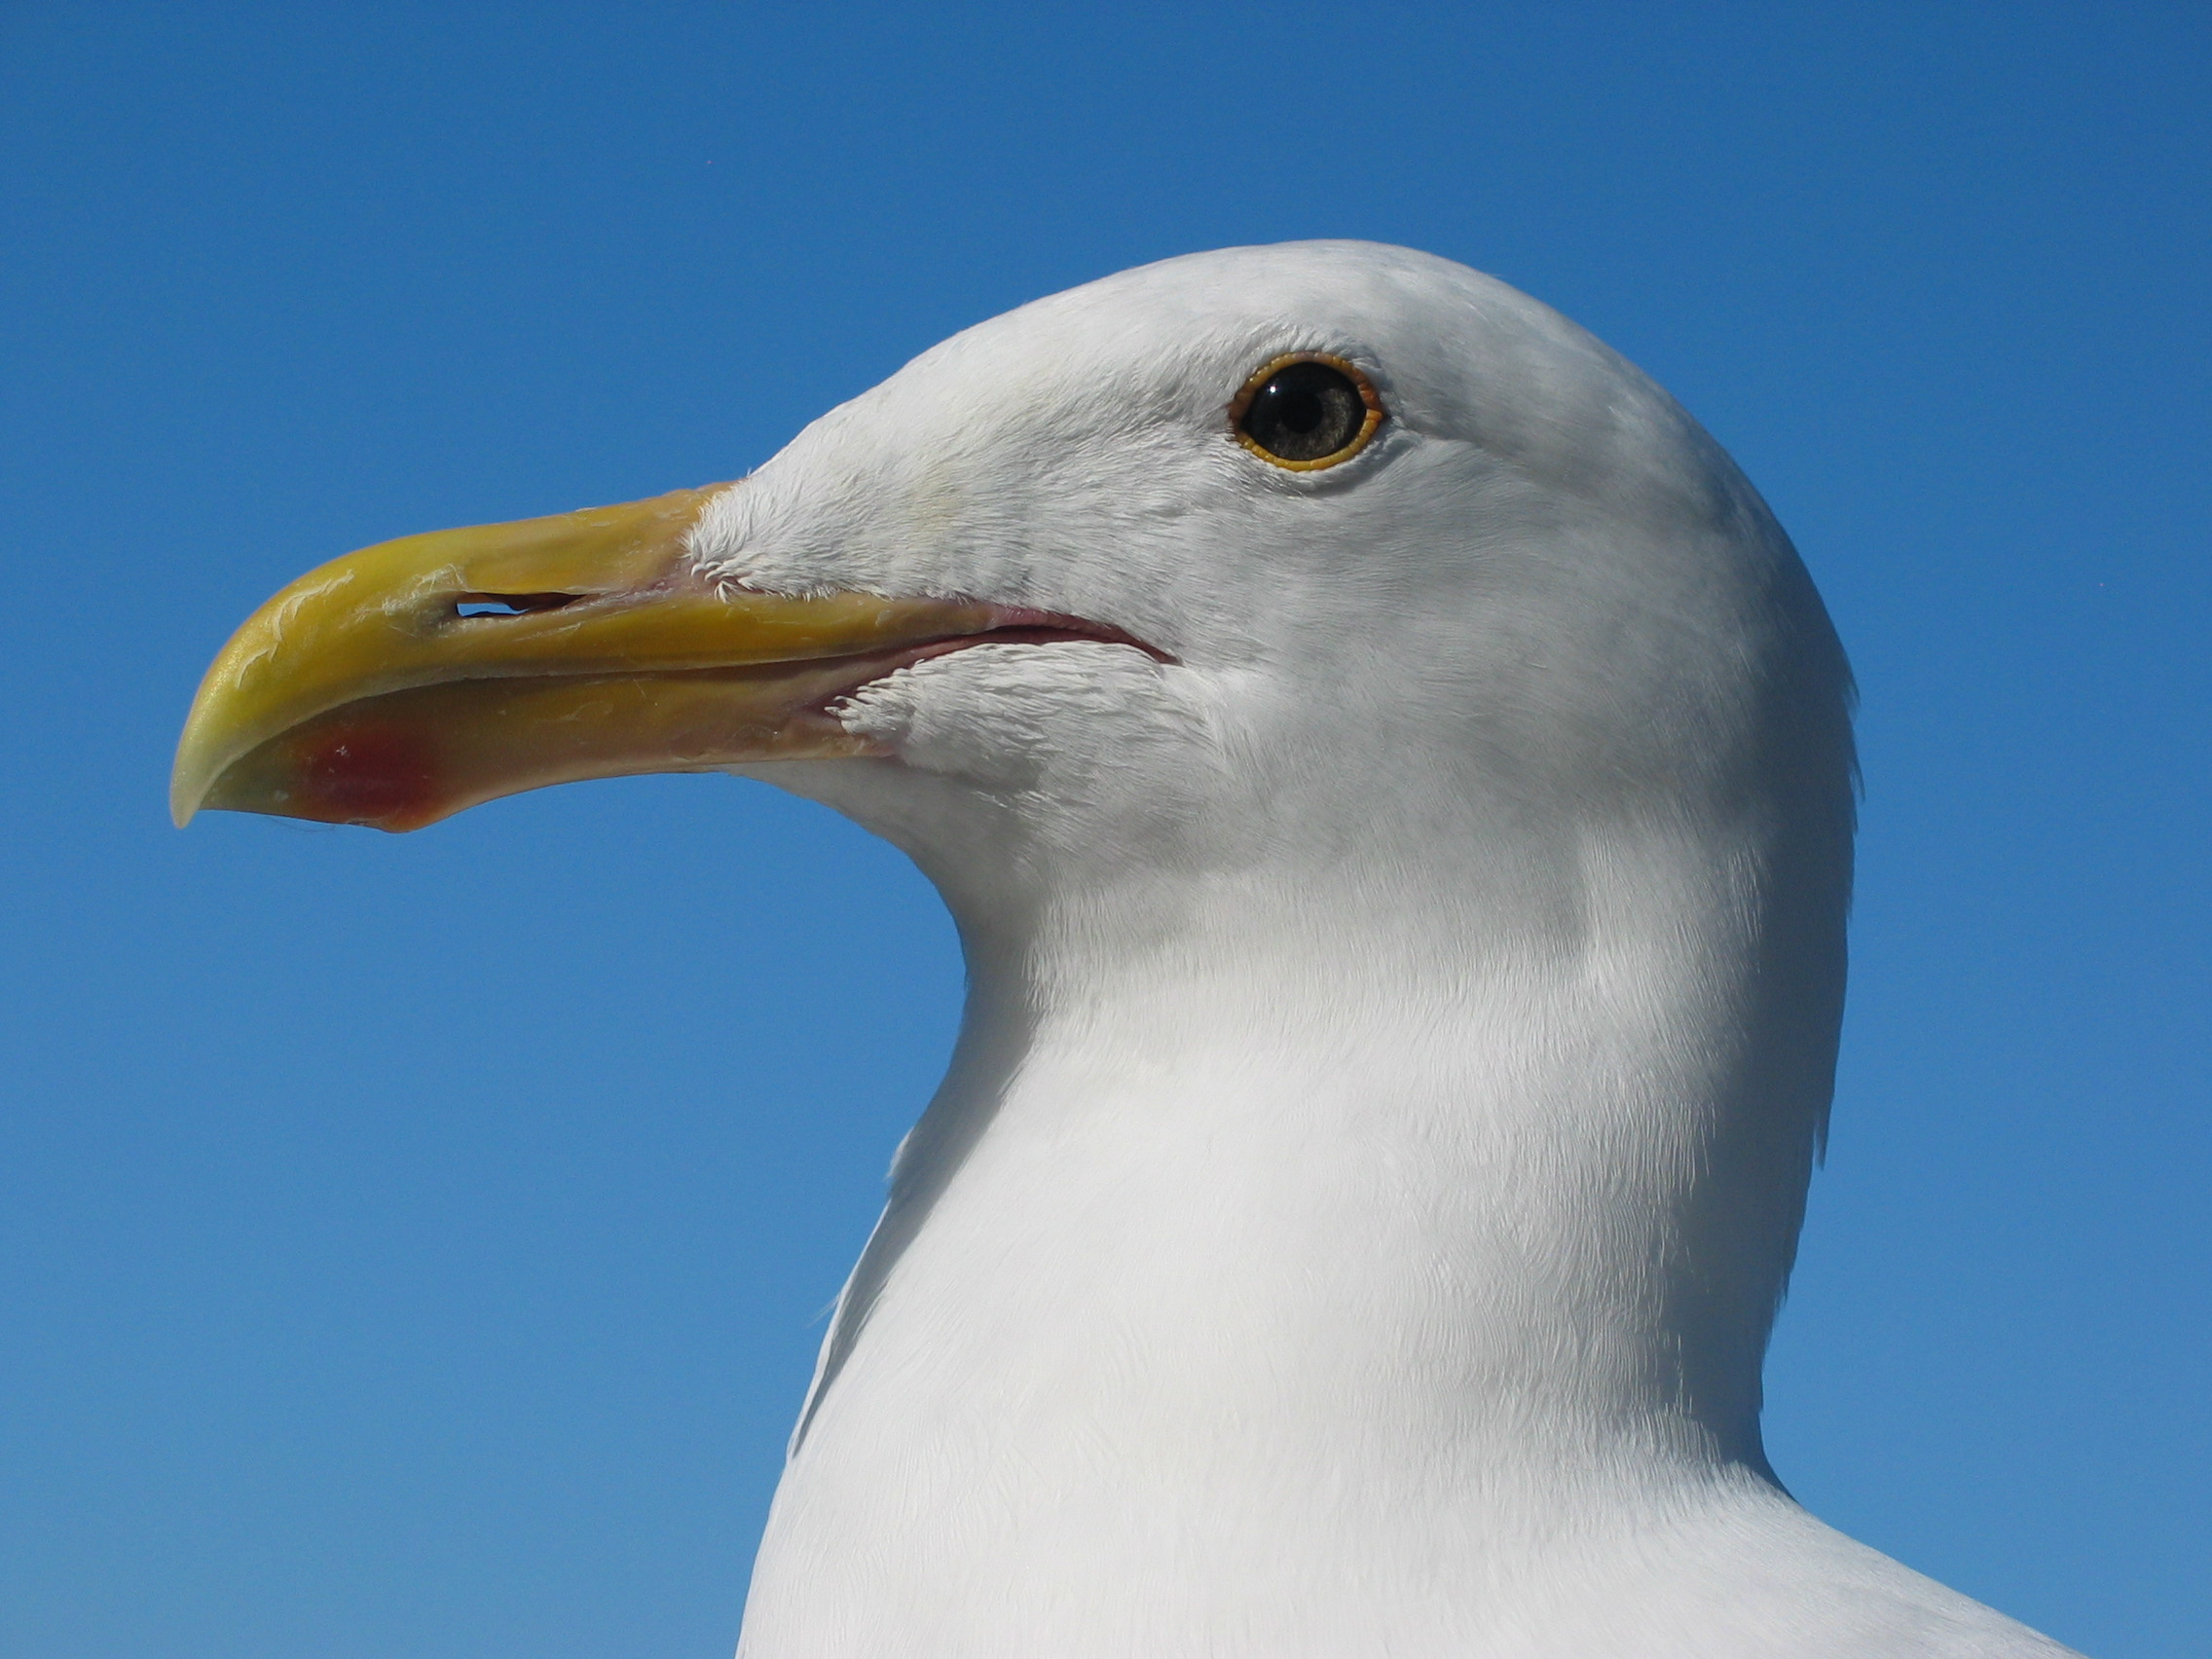
\includegraphics[width=0.8\textwidth]{chapters/images/gull}
  \caption{A picture of a gull.}
\end{figure}

\section{3D geometry}

Yes  - do coordinate systems, transformations, notation
Brief description of SE(3) and SO(3)

\section{Lie Groups}
\label{sec:lie_group}

A Lie group $G$ is a set of elements that must satisfy a number of axioms, mainly; the group must be closed under its binary operation, it must be associative, it must have a unique identity element and each element must have a unique inverse.  A Lie group can be thought of as a manifold, allowing calculus on a local space.  The local neighbourhood of any element can be described by its tangent space, which forms the so called Lie Algebra $\mathfrak g$.  For every element there is an exponential map $\exp\colon \mathfrak g \to G$ that maps from Lie algebra to its Lie Group element.  There also exists a logarithmic map $\log\colon G \to \mathfrak g$.  That maps from the Lie Group element to Lie algebra.
%link to copy formulas:
%https://www.google.com/url?sa=t&rct=j&q=&esrc=s&source=web&cd=1&cad=rja&ved=0CC4QFjAA&url=http%3A%2F%2Fwww.ai.sri.com%2F~agrawal%2Ficcv05.pdf&ei=tzWQUrW_JYqjrgGgyoHgBQ&usg=AFQjCNEf5gEIFxkeoWnymDixktsxuHRilQ&sig2=94gwoKQvghQEIh_nLeAZ8A&bvm=bv.56988011,d.aWM
$SO(3)$

$SE(3)$

provide explanation, mappings

\section{Camera Models}

In order to utilise a camera as a sensor, a mapping between image coordinates and world coordinates needs to be derived.  This allows observations of the camera to be transformed into meaningful measurements.  To achieve this mapping a sensor model of the camera is required. This section will cover all the different types of cameras used in this work and corresponding camera models for each. 

\subsection{Pinhole Camera Model}
\label{subsec:pinhole_cam}

%TODO: references

The pinhole camera model is the most basic and common of camera models used in computer vision.  It describes the mathematical relationship between the coordinates of a 3D point in the world and its projection onto an image plane.  This model assumes the aperture of the camera to be an ideal pinhole. It does not consider lenses used to focus light which in reality result in lense distortion.  It does also not take into account sensor quantization apparent in using a modern digital CCD sensor. Nevertheless it still provides a sufficient model of camera projection for this work, and practical considerations such as image size, resolution and lense distortion can be compensated for.

When using the pinhole camera model, the camera is assumed to be a sealed box with a pinhole aperture on one side, and the image plane, or image sensor on the other side.  Having a small aperture blocks most of the light rays from objects in the world and allows a focused and inverted image of the world to be recorded. In this case the focal point is the aperture and the focal length is the distance from the aperture to the sensor. fig. whatever. For all intensive purposes, this model can be redrawn as in fig. whatever whatever. The image plane is inverted and shown reflected in front the of the camera.  As long as the focal length can be determined, it is then trivial to calculate coordinates on the sensor for a given ray or world coordinate using simple geometry. Sensor coordinates can then be converted to image coordinates given the physical size of the CCD and its resolution.  

Take note the principle point is often not in the sensor of the image, and therefore the coordinates of this point on the sensor needs to be determined.  In addition the focal length varies from camera to camera and therefore both of these values need to be determined by performing an intrinsic calibration. For the calibration, the focal length may be expressed in pixel units, which means the conversion from metric sensor coordinates ( m) to pixel coordinates (u,v) is also performed in one step.

%http://www.jordicenzano.name/projects/2D-to-3D-Paradigm-overview/camera-model
%use this for picture motivation

\begin{figure}[h!]
  \centering
    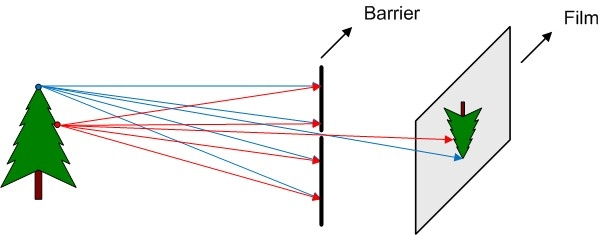
\includegraphics[width=0.5\textwidth]{chapters/images/cam_model_fig2}
  \caption{Pinhole camera model}
\end{figure}

\begin{figure}[h!]
  \centering
    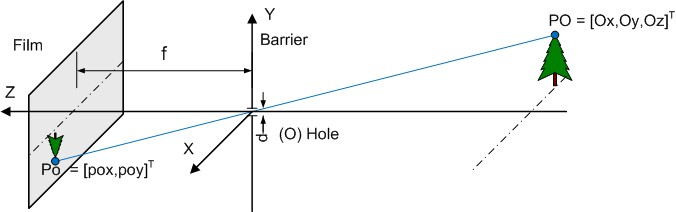
\includegraphics[width=0.9\textwidth]{chapters/images/cam_model_fig41} \\
    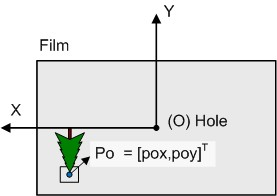
\includegraphics[width=0.3\textwidth]{chapters/images/cam_model_fig42} \\
    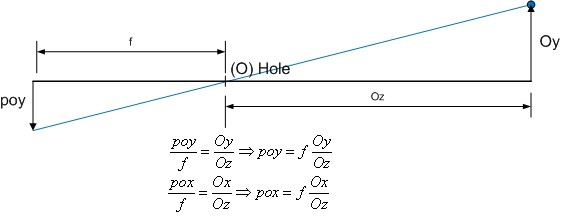
\includegraphics[width=0.9\textwidth]{chapters/images/cam_model_fig43} 
  \caption{Pinhole camera model with image plane shown inverted in front of the focal point}
\end{figure}

%%TODO: I stole these pictures.  I want to redraw them myself

\subsection{Lense Distortion}

%TODO: references

The problem with using a pinhole camera in practice is that it does not allow enough light to into the camera, requiring longer exposure time and therefore blurring in the presence of movement. Therefore a double convex lense is used to focus more light rays onto the sensor and allowing a sharper image.  Such as setup can be seen in fig. xyz.  The pinhole camera model may still be used, however now lense distortion needs to be accounted for.  Lense distortion causes lines to be curved, as in fig x.  It is also possible during the intrinsic calibration to simultaneously determine distortion coefficients which allow the image to be reshaped such that all straight lines appear straight.

\begin{figure}[h!]
  \centering
    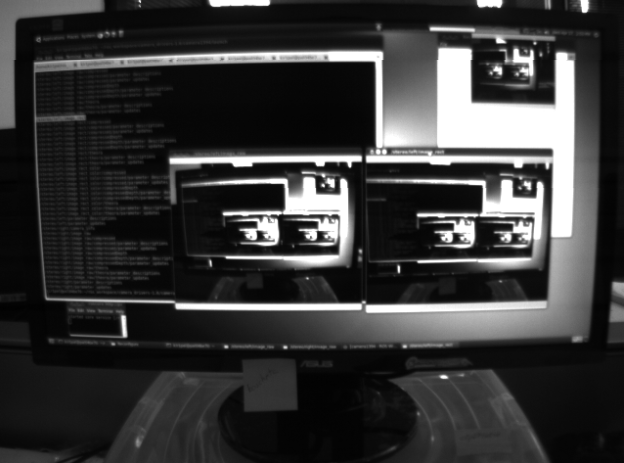
\includegraphics[width=0.49\textwidth]{chapters/images/distorted}
    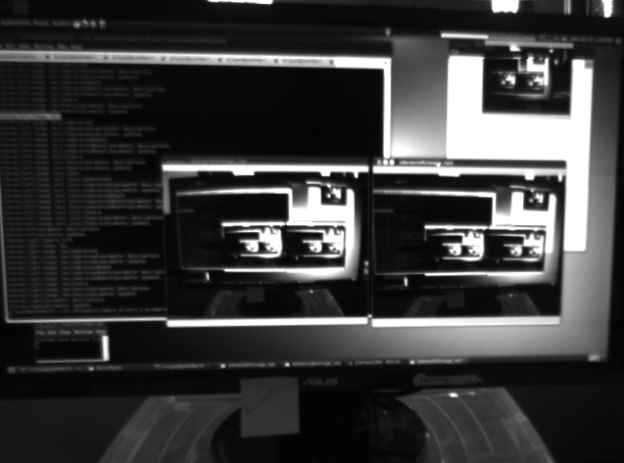
\includegraphics[width=0.49\textwidth]{chapters/images/undistorted}
  \caption{Left: An image with lense distortion.  Right: The same image with lense distortion
compensated for}
\end{figure}

\subsection{Homogeneous coordinates}

%%TODO: homogeneous coordinates

\begin{equation}
 \begin{pmatrix}
  u \\
  v \\
  1 
 \end{pmatrix} =
 \begin{pmatrix}
  f_x & 0 & c_x \\
  0 & f_y & c_y \\
  0 & 0   & 1 
 \end{pmatrix}
 \begin{pmatrix}
  X \\ Y \\ Z
 \end{pmatrix}
\end{equation}


\subsection{Stereo Camera}

\subsection{Omni-directional Camera}

% ask matthias for literature

\subsection{Flir}
Leave this to last.  Flir may (probably) get left out

\section{Computer Vision Basics}

\subsection{Feature point detection and extraction}
\label{subsec:features}

Outline what is feature point detection, description and matching, why we need it.  Mention SIFT and SURF and cite them.  Mention that we used a GPU implemtation of SIFT, cite the ETH paper. Mention a bunch of other descriptors, cite them as well.

\subsection{Reprojection Error}

Reprojection error is an important concept that will be referred to many times in this work.  It is a very powerful tool to more accurately model the cameras accuracy as a sensor.
%TODO

\subsection{RANSAC}
\label{subsec:RANSAC}

explain this cos its easy and fun.  Cite a paper

\subsection{Geometry estimation}

\subsubsection{5 point algorithm}
\label{subsec:5point}
ask for matthias for relavent literature

\subsubsection{Point triangulation}

ask for matthias for relavent literature

\subsubsection{Stereo pose estimation}
\label{subsec:horn}

Umeyama (PCL) \newline 
Horn (UVM)


\section{Place Recognition}

Bag of words

\section{Visual SLAM}

%Cover this in abstract terms.  Talk about the theory, not implemtation.  Mention
%PTAM and cite it.
%No g2o here.

Simulataneous Localization and Mapping (SLAM) is the technique of building a map of a previously
unexplored area whilst simultaneously determining a position (localizing) within that map.  The
traditional approach for SLAM can be split into 4 steps.
\begin{enumerate} \itemsep1pt \parskip0pt \parsep0pt
 \item Feature extraction
 \item Data association
 \item Pose estimation
 \item Global Optimization
\end{enumerate}

%TODO: cite kalman filter
Feature extraction involves finding unique features within the sensor data, also known as landmarks, which can be later in future sensor measurements.  Data association is the process of matching these landmarks over multiple sensor readings, in essence tracking them.  Pose estimation involves using the information of how multiple landmarks moved over time with respect to the robot/sensor in order to determine how the robot moved with respect to those landmarks.  Finally, having determined a map of landmarks, and a pose with respect to those landmarks, a global optimization, or bundle adjustment, over all landmarks and robot poses may be performed in order to produce a globally consistent map and trajectory.  In the past this has commonly been done by using a kalman filter (cite) and by adding all landmarks to the system state. In more recent times graph optimization approaches have become popular as they scale much better to larger maps.

SLAM has taken many forms depending on sensors available. Visual SLAM denotes performing SLAM using some kind of camera.  In recent times, a plethora of visual SLAM algorithms for monocular cameras (cite andrew davidson slam, ptam, something else), stereo cameras (more citations) and RGBD cameras (rgbdslam, kinfu, kintinuous) have been developed.  A keyframe SLAM system similar in concept to the PTAM approach has been utilised as the basis for this work.  The basic operation for this style of SLAM will be outlined here.

\subsection{Basic VSLAM pipeline}

The following is a description of a basic pipeline for visual SLAM.  Whilst the SLAM system that this work is based on is somewhat more complex, this shows how all the above algorithms may be used together to form a complete SLAM pipeline.  The utilised SLAM system will be discussed in section \ref{chapter:ScaViSLAM}

The feature extraction in Visual SLAM involves using image feature detectors/ descriptors as outlined in section \ref{subsec:features}.  These features may then be referred to as landmarks. For a single observation of a landmark from one frame of a single camera, one can determine a 3D ray from the current camera pose by making use of the camera model as outlined in section \ref{subsec:pinhole_cam}.  Multiple observations from multiple frames allows for multiple rays to intersect at this landmark, thus a 3D position of the landmark may be estimated using triangulation. In the case of a stereo camera, the 3D estimate more or less comes for free, as landmarks may be triangulated from left and right camera frame.

The data association stage is performed by doing feature matching across different camera frames. Pose estimation is commonly achieved by utilising the RANSAC algorithm (\ref{subsec:RANSAC}) This can be coupled with the 5 point algorithm (\ref{subsec:5point}) in the case of monocular SLAM (2D-2D correspondances), or with Umeyama/Horn (\ref{subsec:horn}) for stereo or RGBD, (3D-3D correspondances). The model in this case is the 6 DoF transform between frames. The error is calculated by projecting landmarks from one frame to the next by applying the transformation to each of them. The error is then the sum of the distances between points of one frame, and the corresponding points transformed to that same frame. \ref{eq:ransac_error}

\begin{figure}
 \centering
 \begin{math}
  e = \sum\limits_{\bv p_i} \bv p^a_i - ^a\bv T_b \cdot \bv p^b_i
 \end{math}
 \caption{RANSAC error function.  this formula sucks needs formatting}
 \label{eq:ransac_error}
\end{figure}
%TODO: fix formula

Bundle adjustment over all landmarks and camera poses is commonly achieved with a graph optimization. This will be expanded on in sec \ref{subsec:graph_slam}

\subsection{Keyframe SLAM}

The main idea behind keyframe SLAM is to divide the tasks of localization and mapping, and have them run in parallel is separate threads.  The mapping thread defines a keyframe to track against. This amounts to a global pose of the keyframe, as well as a number of landmarks visible from that keyframe recorded relative to that keyframe pose.  The localization thread localizes the camera with respect to that keyframe.  If the camera moves or rotates a significant distance away from the active keyframe, a new keyframe will be created with a known transformation to the previous keyframe.

The intent is to have a fast localization thread that runs in realtime providing an accurate pose estimation with respect to the keyframe.  The mapping thread that deals with the keyframe runs at a much lower framerate, and handles changing the keyframe, global optimization(?), something else. The overall outcome is a system that provides an accurate pose in global coordinates with a fast update rate, as well as a globally consistent map.
%TODO: read PTAM paper again.  You do not know what the hell you are on about here

\subsection{Loop Closure}
\label{subsec:loop_closure}

A common problem with visual SLAM systems is that the pose estimation between frames is not perfectly accurate.  While locally this is not a problem, if the camera is to move a long distance this error will accumulate, as the current pose is a product of all the previous frame to frame transformations.  This effect can easily be demonstrated by performing a long trajectory and returning to the start point.  Whilst the camera is in its original position, the estimated pose will be some offset from the origin.

\begin{figure}[h!]
  \centering
    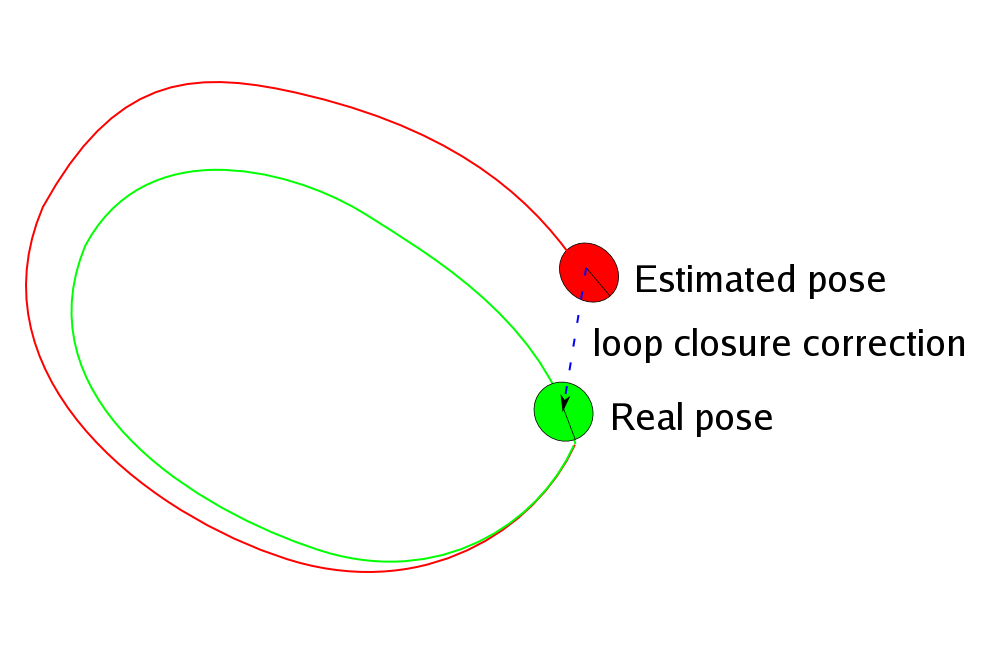
\includegraphics[width=0.5\textwidth]{chapters/images/loop-closure}
  \caption{Loop Closure}
\end{figure}

It is possible to compensate for this visual odometry drift by performing 'large loop closures'. After returning to a previous location, the current frame can be registered against an earlier recorded frame at this location using the standard pipeline of pose estimation based on shared landmark observations.  The current pose may be corrected to the correct position by adjusting all of the previous poses slightly.  This adjustment may be performed efficiently and optimally using graph optimization.

\section{Graph SLAM}
\label{subsec:graph_slam}

To express an optimization problem as a graph, one can think of vertices as being variables, or states, to optimize over, and edges as being constraints for 1 or more vertices.  Edges for a single vertex are called unary edges, for two vertices binary edges and more than 2 multi edges.  Vertex states may be one or more dimensions.  Having said that, vertices may also be used as parameters in the optimization problem.  Error functions to minimise are then defined as how well vertex states fit their edge constraints.  Due to the fact an edge may connect more than two vertices, this type of graph is referred to as a hyper-graph.

An example of how a simple SLAM problem may be expressed as a hyper-graph is shown below.
\begin{figure}[h]
  \centering
      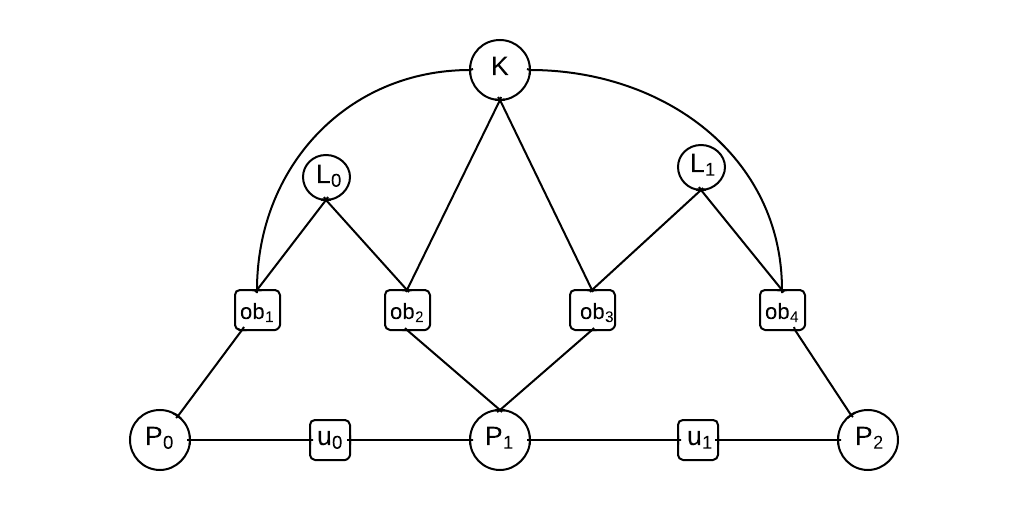
\includegraphics[width=1.0\textwidth]{chapters/images/simple_slam}
  \caption{A simple SLAM graph for a generic robot.  Circles are vertices to optimize over, and
squares are edges, which in this case are measurements}
\end{figure}

The diagram shows robot poses as $\bv P_i$.  These poses could be represented by any number of dimensions. In the case of an exploratory robot, this is likely to be 3 dimensional (x, y, and yaw for movement on a fixed plane), or 6 dimensional (x, y, z, rotation about x, rotation about y, rotation about z).  $\bv U_i$ are binary edges, representing odometry measurements between robot poses. These are measurements or constraints and will remain unchanged during optimization.  
$\bv L_i$ represents unique landmarks that the robot can sense and make some form of measurement relative to its own position, as well as re-identify in different robot poses.  A landmark could be a corner from a laser scan or a feature point in a camera image.  K represents calibration parameters of the sensor.  This could be something like an offset, camera intrinsic parameters, or an extrinsic parameter to transform the sensor readings from the sensor frame to the robot frame.  $\bv {ob}_i$ are observation multi-edges, between a robot pose, a landmark, and the calibration parameter.

Such an example of graph optimization would allow an optimization of the poses of the robot, positions of the landmarks, and the sensor calibration, based on all odometry and observation measurements.

In order to compute this optimization, the generic graph problem may be represented mathematically as follows:

 \begin{align}
   \bv{F}(\bv x) &= \sum\limits_{K \in C}^{} 
                 \bv e_k(\bv x_k, \bv z_k)^T 
                 \bv \Omega_k
                 \bv e_k(\bv x_k, \bv z_k)  \\ 
   \bv x^* &= \operatornamewithlimits{argmin}\limits_{\bv x}\bv{F}(\bv x)
 \end{align}

\begin{itemize}
 \item $\bv x$ is a vector of parameter sets, whereby each $\bv x_i$ is a parameter block
 \item $\bv x_k$ is a set of parameters involved in the $k$th constraint
 \item $\bv z_k$ is a constraint or measurement relating to parameter $\bv x_k$
 \item $\bv \Omega_k$ is the information matrix for $\bv z_k$.  This can be used to weight this constraint
 \item $\bv e_k(\bv x_k, \bv z_k)$ is the error function that measures how well parameter block $\bv x_k$ satisfies $\bv z_k$.  If for instance $\bv z_k$ directly measured $\bv x_k$, then a straightforward error function would be $\bv e_k(\bv x_k, \bv z_k) = \bv x_k - \bv z_k $
\end{itemize}

\subsection{Solving the least squares problem}

%TODO: citations
A numerical solution to eq. 4.2 can be performed using a non linear solver such as Gauss-Newton or Levenberg-Marquardt (cite, cite).  The error function can be approximated by its first order Taylor expansion around the current initial guess $\breve{\bv x}$

\begin{align}
  \bv e_k(\breve{\bv x}_k + \Delta \bv x_k) &= \bv e_k(\breve{\bv x} + \Delta \bv x) \\
      & \simeq \bv e_k + \bv J_k \Delta \bv x
\end{align}

$\bv J_k$ is the Jacobian of $\bv e_k(\bv x)$ computed in $\breve{\bv x}$.  Substituting eq(4.4) as the error function in eq(4.1), one obtains:

\begin{align}
  \bv F(\breve{\bv x} + \Delta \bv x) &= \bv e_k(\breve{\bv x} + \Delta \bv x)^T \bv \Omega_k \bv e_k(\breve{\bv x} + \Delta \bv x) \\
  & \simeq (\bv e_k + \bv J_k \Delta \bv x)^T 
    \bv \Omega_k 
    (\bv e_k + \bv J_k \Delta \bv x) \\
  &= \bv e_k^T \bv \Omega_k \bv e_k 
    + 2 \bv e_k^T \bv \Omega_k \bv J_k \Delta \bv x 
    + \Delta \bv x^T \bv J_k^T \bv \Omega_k \bv J_k \Delta \bv x \\
  &= c_k + 2\bv b_k \Delta \bv x + \Delta \bv x \bv H_k \Delta \bv x
\end{align}

Where $c_k = \bv e_k^T \bv \Omega_k \bv e_k$, $\bv b_k = \bv e_k^T \bv \Omega_k \bv J_k$ and $\bv H_k = \bv J_k^T \bv \Omega_k \bv J_k$. This quadratic form can then be minimized in $\Delta \bv x$ by solving the linear system

\begin{align}
   \bv H \Delta \bv x^* = -\bv b
\end{align}

$\bv H$ is a very large sparse square matrix.  It is mostly zeros; it only contains non zero values where there is a constraint connecting blocks.  This matrix can be efficiently solved by taking advantage of the fact that is is sparse, for instance, by Cholesky factorization.

\subsection{Operator to apply increments in optimization}
%TODO: oplus fill in 
As part of the SLAM problem, it is common to have parameterization in non Euclidean space.  For instance, a 3 dimensional pose $SE(3)$ is described by a translational part $\mathbb{R}^3$, which is clearly Euclidean, and a rotational component $SO(3)$ which is not euclidean.  The rotation part is often described in some over parameterized way, for instance quaternions or rotational matrices.  

The solver is mostly likely to be agnostic about the exact representation of the vertex state, it just knows the degrees of freedom of a vertex.  This means during optimization the optimizer will provide increments to the vertex in the form of a vector with as many values as degrees of freedom.  If the rotational part was expressed as a rotation matrix, then somehow this 3D vector needs to be applied to the matrix in a sensible way.  The vector may not be simply added or multiplied to the matrix due to the non euclidean nature of this representation.

One way to deal with this is to optimize over all degrees of freedom of the over parameterized representation, in this case 9 degrees for an $SO(3)$ + 3 for the translation part, therefore 12 degrees per vertex, however this makes the problem more complex and can introduce error.  Another way is to use the 3D increment vector as Euler angles, however singularities could occur due to Gimbal lock.

A better idea is to consider the problem space as a manifold.  A manifold is a space that globally may not be euclidean, although locally can be considered euclidean.  Then one needs to define an operator, denoted $\boxplus$, which maps a local variation $\Delta\bv x$ in Euclidean space on to the Manifold. $\bv e_k(\bv x_k \boxplus \Delta\bv x$)

The Lie algebra provides a compact representation of the element, and therefore we can use the exponential map $\exp\colon \mathfrak g \to G$ for the $\boxplus$ operator.  For a further explanation of Lie groups and the logarithmic map, please see \ref{sec:lie_group}

\subsection{Error functions}

The error function $\bv e_k(\bv x_k, \bv z_k)$ measures how well the vertices fit the the edge that they are connected to.  A similar problem is encountered as for vertex increments when calculating error for the case of non euclidean parameterization.  Again for the example of the $SE(3)$ pose, in this case the error, which could be described as an $SE(3)$ pose, needs to be converted to some minimal vector form for the optimizer.  In this case the  logarithmic mapping $\log\colon G \to \mathfrak g$ can be used to achieve this conversion. More details see \ref{sec:lie_group}

%\subsubsection{Robust least squares}
%TODO huber fill in
%Use huber instead of squares to make robust against outliers. !
%CBF
